%\chapter{Cap\'{\i}tulo 2}
%Existen varias normas para la citaci\'{o}n bibliogr\'{a}fica. Algunas \'{a}reas del conocimiento prefieren normas espec\'{\i}ficas para citar las referencias bibliogr\'{a}ficas en el texto y escribir la lista de bibliograf\'{\i}a al final de los documentos. Esta plantilla brinda la libertad para que el autor de la tesis  o trabajo de investigaci\'{o}n utilice la norma bibliogr\'{a}fica com\'{u}n para su disciplina. Sin embargo, se solicita que la norma seleccionada se utilice con rigurosidad, sin olvidar referenciar "todos" los elementos tomados de otras fuentes (referencias bibliogr\'{a}ficas, patentes consultadas, software empleado en el manuscrito, en el tratamiento a los datos y resultados del trabajo, consultas a personas (expertos o p\'{u}blico general), entre otros).\\
%
%\section{Ejemplos de citaciones bibliogr\'{a}ficas}
%Existen algunos ejemplos para la citaci\'{o}n bibliogr\'{a}fica, por ejemplo, Microsoft Word (versiones posteriores al 2006), en el  men\'{u} de referencias, se cuenta con la opci\'{o}n de insertar citas bibliogr\'{a}ficas utilizando la norma APA (American Psychological Association) u otras normas y con la ayuda para construir autom\'{a}ticamente la lista al final del documento. De la misma manera, existen administradores bibliogr\'{a}ficos compatibles con Microsoft Word como Zotero, End Note y el Reference Manager,  disponibles a trav\'{e}s del Sistema Nacional de Bibliotecas (SINAB) de la Universidad Nacional de Colombia\footnote{Ver:www.sinab.unal.edu.co } secci\'{o}n "Recursos bibliogr\'{a}ficos" opci\'{o}n "Herramientas Bibliogr\'{a}ficas. A continuaci\'{o}n se muestra un ejemplo de una de las formas m\'{a}s usadas para las citaciones bibliogr\'{a}ficas.\\
%
%Citaci\'{o}n individual:\cite{AG01}.\\
%Citaci\'{o}n simult\'{a}nea de varios autores:
%\cite{AG12,AG52,AG70,AG08a,AG09a,AG36a,AG01i}.\\
%
%Por lo general, las referencias bibliogr\'{a}ficas correspondientes a los anteriores n\'{u}meros, se listan al final del documento en orden de aparici\'{o}n o en orden alfab\'{e}tico. Otras normas de citaci\'{o}n incluyen el apellido del autor y el a\~{n}o de la referencia, por ejemplo: 1) "...\'{e}nfasis en elementos ligados al \'{a}mbito ingenieril que se enfocan en el manejo de datos e informaci\'{o}n estructurada y que seg\'{u}n Kostoff (1997) ha atra\'{\i}do la atenci\'{o}n de investigadores dado el advenimiento de TIC...", 2) "...Dicha afirmaci\'{o}n coincide con los planteamientos de Snarch (1998), citado por Castellanos (2007), quien comenta que el manejo..." y 3) "...el futuro del sistema para argumentar los procesos de toma de decisiones y el desarrollo de ideas innovadoras (Nosella \textsl{et al}., 2008)...".\\
%
%\section{Ejemplos de presentaci\'{o}n y citaci\'{o}n de figuras}
%Las ilustraciones forman parte del contenido de los cap\'{\i}tulos. Se deben colocar en la misma p\'{a}gina en que se mencionan o en la siguiente (deben siempre mencionarse en el texto).\\
%
%Las llamadas para explicar alg\'{u}n aspecto de la informaci\'{o}n deben hacerse con nota al pie y su nota correspondiente\footnote{Las notas van como "notas al pie". Se utilizan para explicar, comentar o hacer referencia al texto de un documento, as\'{\i} como para introducir comentarios detallados y en ocasiones para citar fuentes de informaci\'{o}n (aunque para esta opci\'{o}n es mejor seguir en detalle las normas de citaci\'{o}n bibliogr\'{a}fica seleccionadas).}. La fuente documental se debe escribir al final de la ilustraci\'{o}n o figura con los elementos de la referencia (de acuerdo con las normas seleccionadas) y no como pie de p\'{a}gina. Un ejemplo para la presentaci\'{o}n y citaci\'{o}n de figuras, se presenta a continuaci\'{o}n (citaci\'{o}n directa):\\
%
%Por medio de las propiedades del fruto, seg\'{u}n el espesor del endocarpio, se hace una clasificaci\'{o}n de la palma de aceite en tres tipos: Dura, Ternera y Pisifera, que se ilustran en la Figura
%\ref{fig:Fruto}.\\
%\begin{figure}[h]
%\centering%
%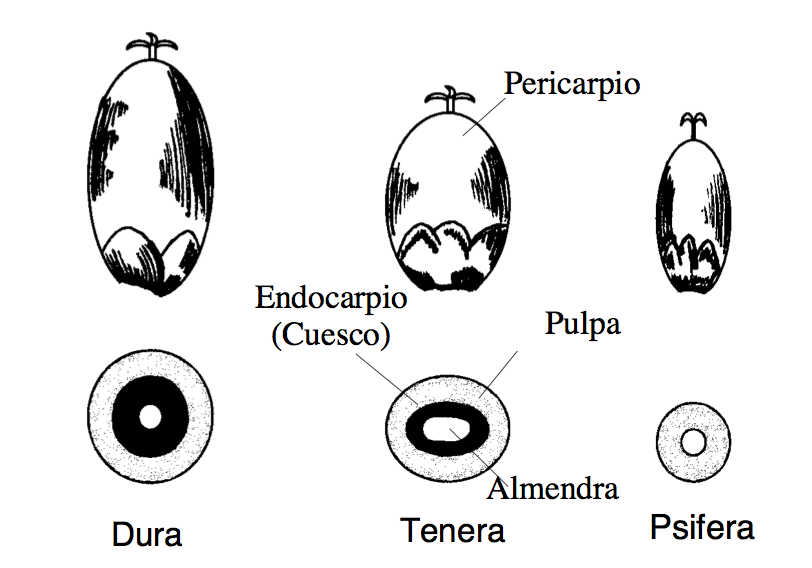
\includegraphics{Kap3/FrutoSp}%
%\caption{Tipos y partes del fruto de palma de aceite \cite{AG03p,AG04p}.} \label{fig:Fruto}
%\end{figure}
%
%\section{Ejemplo de presentaci\'{o}n y citaci\'{o}n de tablas y cuadros}
%Para la edici\'{o}n de tablas, cada columna debe llevar su t\'{\i}tulo; la primera palabra se debe escribir con may\'{u}scula inicial y preferiblemente sin abreviaturas. En las tablas y cuadros, los t\'{\i}tulos y datos se deben ubicar entre l\'{\i}neas horizontales y verticales cerradas (como se realiza en esta plantilla).\\
%
%La numeraci\'{o}n de las tablas se realiza de la misma manera que las figuras o ilustraciones, a lo largo de todo el texto. Deben llevar un t\'{\i}tulo breve, que concreta el contenido de la tabla; \'{e}ste se debe escribir en la parte superior de la misma. Para la presentaci\'{o}n de cuadros, se deben seguir las indicaciones dadas para las tablas.\\
%
%Un ejemplo para la presentaci\'{o}n y citaci\'{o}n de tablas (citaci\'{o}n indirecta), se presenta a continuaci\'{o}n:\\
%
%De esta participaci\'{o}n aproximadamente el 60 \% proviene de biomasa
%(Tabla \ref{EMundo1}).
%\begin{center}
%\begin{threeparttable}
%\centering%
%\caption{Participaci\'{o}n de las energ\'{\i}as renovables en el suministro
%total de energ\'{\i}a primaria \cite{AG02i}.}\label{EMundo1}
%\begin{tabular}{|l|c|c|}\hline
%&\multicolumn{2}{c|}{Participaci\'{o}n en el suministro de energ\'{\i}a primaria /\% (Mtoe)\;$\tnote{1}$}\\\cline{2-3}%
%\arr{Region}&Energ\'{\i}as renovables &Participaci\'{o}n de la biomasa\\\hline%
%Latinoam\'{e}rica&28,9 (140)&62,4 (87,4)\\\hline%
%\:Colombia&27,7 (7,6)&54,4 (4,1)\\\hline%
%Alemania&3,8 (13,2)&65,8 (8,7)\\\hline%
%Mundial&13,1 (1404,0)&79,4 (1114,8)\\\hline
%\end{tabular}
%\begin{tablenotes}
%\item[1] \footnotesize{1 kg oe=10000 kcal=41,868 MJ}
%\end{tablenotes}
%\end{threeparttable}
%\end{center}
%
%NOTA: en el caso en que el contenido de la tabla o cuadro sea muy extenso, se puede cambiar el tama\~{n}o de la letra, siempre y cuando \'{e}sta sea visible por el lector.\\
%
%\subsection{Consideraciones adicionales para el manejo de figuras y tablas}
%Cuando una tabla, cuadro o figura ocupa m\'{a}s de una p\'{a}gina, se debe repetir su identificaci\'{o}n num\'{e}rica, seguida por la palabra continuaci\'{o}n.\\
%
%Adicionalmente los encabezados de las columnas se deben repetir en todas las p\'{a}ginas despu\'{e}s de la primera.\\
%
%Los anteriores lineamientos se contemplan en la presente plantilla.\\
%
%\begin{itemize}
%\item Presentaci\'{o}n y citaci\'{o}n de ecuaciones.
%\end{itemize}

%La citaci\'{o}n de ecuaciones, en caso que se presenten, debe hacerse como lo sugiere esta plantilla. Todas las ecuaciones deben estar numeradas y citadas detro del texto.\\

%Para el manejo de cifras se debe seleccionar la norma seg\'{u}n el \'{a}rea de conocimiento de la tesis  o trabajo de %investigaci\'{o}n.\\

%\chapter{Theoretical Framework}
\chapter{Planteamiento del Problema}
%
\section{Antecedentes}

A continuación se mencionan los autores que presentan modelos matemáticos en el área de la simulación de procesos de recobro mejorado e ilustran el dominio de aplicación con diversas representaciones. \cite{ValenciaJD2016, valencia2018development} desarrollan un modelo de simulación para la generación de espumas \textit{in situ} inyectando químicos dispersos en gas. En este trabajo, describen los fenómenos físicos y mecanismos, de los fluidos y del químico inyectado, que se presentan en el yacimiento. Adicionalmente, presentan las ecuaciones de su modelo matemático y un diagrama de flujo del proceso de solución de las mismas. Sin embargo, los conceptos que se enuncian en su modelo conceptual y matemático no son trazables en sus diagramas y no tienen representación de los eventos que resultan de los fenómenos físicos que se modelan.\\

\cite{MozoID2017} elabora un modelo de inyección de nanopartículas para la estimulación de pozos. En su trabajo, emplea un modelo conceptual para explicar los fenómenos que se describen en su modelo matemático, además, explica el proceso de solución de las ecuaciones de su modelo por medio de un algoritmo. Este trabajo también carece de trazabilidad en los conceptos que se explican. \cite{IsazaCN2017} desarrolla un modelo de remediación del daño generado por asfaltenos, en este se presenta el modelo conceptual para una simulación de tipo \textit{Black Oil} agregándole el transporte de los asfaltenos en el petróleo y su transferencia a la roca. En éste trabajo, también se presenta un algoritmo genérico de solución de las ecuaciones que se muestran en el modelo matemático.\\

Por último, \cite{solano2019modeling}, presenta un modelo de generación de espumas para aplicación en yacimientos naturalmente fracturados, en este trabajo se desarrolla un \textit{Black Oil Model} con inyección de un surfactante disperso en una corriente de gas. Para describir los fenómenos físicos que \cite{solano2019modeling} modelan en el trabajo, presentan un mapa conceptual y las ecuaciones de su modelo matemático. Este trabajo carece de trazabilidad en el proceso de solución de las ecuaciones.\\

Los siguientes autores elaboran \textit{frameworks} de simulación de yacimientos de petróleo. Sus esfuerzos, en su mayoría, se enfocan en la velocidad de computo y procesamiento paralelo. \cite{Zaza2016} presenta un simulador Black Oil en paralelo utilizando la arquitectura CUDA. En este trabajo, \cite{Zaza2016} muestra en un diagrama general, la descripción de cómo se resuelven las ecuaciones de su modelo matemático, involucrando los conceptos que se relacionan con cada etapa de la solución. En éste trabajo, también se muestra el esquema de solución, involucrando conceptos del modelo matemático. Sin embargo, no todos los conceptos son trazables en su esquema de solución.\\

\cite{Wang2016, Wang2017} desarrolla un simulador \textit{Black Oil} en paralelo para múltiples dominios continuos que considera modelos de fracturas discretas en yacimientos no convencionales. En este trabajo se presentan todas las ecuaciones del modelo matemático que relaciona los múltiples dominios, aunque carece de representaciones que agrupen los conceptos, fenómenos físicos y procesos de solución. \cite{FANG2017} desarrollan un modelo flujo entre dos dominios para un sólo fluido. En éste, se calcula un sistema de mallas mezcladas y se definen términos de transmisividad media y total para las transferencias del fluido entre los dominios. En este trabajo, se ilustra un diagrama del proceso de solución de los dos dominios de flujo. Sin embargo, este no acopla todos los conceptos que se definen. \cite{Qiao2017} presentan un \textit{framework} multipropósito basado en un modelo composicional para flujo reactivo, en éste desarrollan todo el modelo matemático y explican cómo acoplar nuevos fenómenos. Sin embargo, no tienen elementos de trazabilidad de conceptos ni del proceso de solución de sus ecuaciones.\\

\cite{Flemisch2011} desarrollan un \textit{framework} de simulación de yacimientos sobre DUNE \citep{DUNE24:16}. La herramienta tiene la capacidad de simular flujo en dos fases con un modelo de múltiples medios continuos (MINC). Las variables de los modelos se pueden resolver de manera completamente implícita y acoplada o de manera secuencial. En su trabajo presentan una representación del proceso con los detalles de implementación de los modelos. Sin embargo, no existen elementos que permitan trazar los conceptos presentes en sus modelos matemáticos. \\

Existen otros trabajos como los de \cite{Cao2002}, \cite{DeBaun2005} y \cite{ZHANG2007135} que tienen elementos de trazabilidad tanto de conceptos como del proceso. Sin embargo, estos son específicos de la manera en la que implementan sus \textit{frameworks}. Adicionalmente carecen de elementos para representar eventos que emergen de los fenómenos físicos que se estudian.\\

En tabla \ref{tab:LitReview} se muestra una síntesis de la revisión de literatura de modelos ejecutables para la simulación de yacimientos de petróleo. Se destaca que existen algunos elementos de trazabilidad, tanto conceptual como del proceso, en los trabajos que se revisan. Sin embargo, faltan elementos de acople que garanticen la cohesión y consistencia de los modelos matemáticos con el método de solución de los mismos. También se evidencia que los trabajos carecen de representación de los eventos que surgen de caracterizar los fenómenos físicos que se estudian en cada trabajo. \\

\begin{table}[h]
	\centering
	\begin{tabular}{|l|l|l|l|l|}
		\hline
		\multicolumn{1}{|c|}{\multirow{2}{*}{\textbf{AUTORES}}} & \multicolumn{4}{c|}{\textbf{Enfoques}}                                                                                                                                                                                                                                                      \\ \cline{2-5} 
		\multicolumn{1}{|c|}{}                         & \begin{tabular}[c]{@{}l@{}}Modelos \\ matemáticos\end{tabular} & \begin{tabular}[c]{@{}l@{}}Trazabilidad \\ de conceptos\end{tabular} & \begin{tabular}[c]{@{}l@{}}Trazabilidad \\ del proceso\end{tabular} & \begin{tabular}[c]{@{}l@{}}Representación \\ de eventos\end{tabular} \\ \hline
		\cite{ValenciaJD2016}                                   & \multicolumn{1}{c|}{x}                                         & \multicolumn{1}{c|}{}                                               & \multicolumn{1}{c|}{}                                              & \multicolumn{1}{c|}{}                                               \\ \hline
		\cite{valencia2018development}                                   & \multicolumn{1}{c|}{x}                                         & \multicolumn{1}{c|}{}                                               & \multicolumn{1}{c|}{}                                              & \multicolumn{1}{c|}{}                                               \\ \hline
		\cite{MozoID2017}                                   & \multicolumn{1}{c|}{x}                                         & \multicolumn{1}{c|}{}                                               & \multicolumn{1}{c|}{x}                                              & \multicolumn{1}{c|}{}                                               \\ \hline
		\cite{IsazaCN2017}                                   & \multicolumn{1}{c|}{x}                                         & \multicolumn{1}{c|}{}                                               & \multicolumn{1}{c|}{x}                                              & \multicolumn{1}{c|}{}                                               \\ \hline
		\cite{solano2019modeling}                                   & \multicolumn{1}{c|}{x}                                         & \multicolumn{1}{c|}{x}                                               & \multicolumn{1}{c|}{}                                              & \multicolumn{1}{c|}{}                                               \\ \hline
		\cite{Zaza2016}                                   & \multicolumn{1}{c|}{x}                                         & \multicolumn{1}{c|}{}                                               & \multicolumn{1}{c|}{x}                                              & \multicolumn{1}{c|}{}                                               \\ \hline
		\cite{Wang2016, Wang2017}                                   & \multicolumn{1}{c|}{x}                                         & \multicolumn{1}{c|}{}                                               & \multicolumn{1}{c|}{}                                              & \multicolumn{1}{c|}{}                                               \\ \hline
		\cite{FANG2017}                                   & \multicolumn{1}{c|}{x}                                         & \multicolumn{1}{c|}{}                                               & \multicolumn{1}{c|}{x}                                              & \multicolumn{1}{c|}{}                                               \\ \hline
		\cite{Qiao2017}                                   & \multicolumn{1}{c|}{x}                                         & \multicolumn{1}{c|}{}                                               & \multicolumn{1}{c|}{}                                              & \multicolumn{1}{c|}{}                                               \\ \hline
		\cite{Flemisch2011}                                   & \multicolumn{1}{c|}{x}                                         & \multicolumn{1}{c|}{}                                               & \multicolumn{1}{c|}{x}                                              & \multicolumn{1}{c|}{}                                               \\ \hline
		\cite{Cao2002}                                   & \multicolumn{1}{c|}{x}                                         & \multicolumn{1}{c|}{x}                                               & \multicolumn{1}{c|}{x}                                              & \multicolumn{1}{c|}{}                                               \\ \hline
		\cite{DeBaun2005}                                   & \multicolumn{1}{c|}{x}                                         & \multicolumn{1}{c|}{x}                                               & \multicolumn{1}{c|}{x}                                              & \multicolumn{1}{c|}{}                                               \\ \hline
		\cite{Mohammad2017}                                  & \multicolumn{1}{c|}{x}                                         & \multicolumn{1}{c|}{}                                               & \multicolumn{1}{c|}{}                                              & \multicolumn{1}{c|}{}                                               \\ \hline
		\cite{WANG201519}                                   & \multicolumn{1}{c|}{x}                                         & \multicolumn{1}{c|}{}                                               & \multicolumn{1}{c|}{}                                              & \multicolumn{1}{c|}{}                                               \\ \hline
		\cite{ZHANG2007135}                                   & \multicolumn{1}{c|}{x}                                         & \multicolumn{1}{c|}{x}                                               & \multicolumn{1}{c|}{x}                                              & \multicolumn{1}{c|}{}                                               \\ \hline
		\cite{Wang2016Pol}                                   & \multicolumn{1}{c|}{x}                                         & \multicolumn{1}{c|}{}                                               & \multicolumn{1}{c|}{}                                              & \multicolumn{1}{c|}{}                                               \\ \hline
		\cite{Hu2013}                                   & \multicolumn{1}{c|}{x}                                         & \multicolumn{1}{c|}{}                                               & \multicolumn{1}{c|}{}                                              & \multicolumn{1}{c|}{}                                               \\ \hline
		\cite{ZAYDULLIN201451}                                   & \multicolumn{1}{c|}{x}                                         & \multicolumn{1}{c|}{}                                               & \multicolumn{1}{c|}{}                                              & \multicolumn{1}{c|}{}                                               \\ \hline
		
	\end{tabular}
\caption[Síntesis de la revisión de literatura.]{Síntesis de la revisión de literatura. Los autores.}
\label{tab:LitReview}
\end{table}


%, que se generan durante la inyección de espumantes dispersos, por medio de un diagrama en el que sólo se mencionan los fenómenos y se agrupan sus mecanismos. 

\section{Problema}
%(Hablar de los esquemas preconceptuales como modelos ejecutables).

La simulación de procesos de recobro mejorado requiere la elaboración y solución de modelos matemáticos complejos \citep{ertekin2001basic}. Éstos involucran múltiples conceptos que describen los fenómenos físicos, y, que pueden estar presentes en diferentes ecuaciones. Las ecuaciones, a pesar de ser una representación formal, no contienen toda la información relevante a la simulación, por lo que se pierde la trazabilidad de los conceptos que se requieren para representar los fenómenos físicos correctamente. Adicionalmente, existe diversidad de técnicas para solucionar los modelos matemáticos que se elaboran. Por ésta razón, hay poca trazabilidad en los procesos de solución. Todo esto repercute en que los simuladores de yacimientos para procesos EOR se desarrollen de manera empírica, sin seguir un estándar.\\

Los esquemas preconceptuales son una herramienta que permite representar dominios de conocimiento. Estos, mantienen la cohesión de los elementos presentes en un dominio, puesto que agrupan toda su estructura. Adicionalmente, el mismo esquema sirve para representar el comportamiento dinámico o los procesos que se dan en dicho dominio. Recientes trabajos, muestran el potencial de los esquemas preconceptuales para representar dominios de aplicación en el área del software científico.\\

Por ejemplo, \cite{norena2018timrep} representan eventos temporales usando EPs, y lo ejemplifican con la simulación de un sensor que toma mediciones de temperatura constantemente y modifica el estado de una alerta. Más aún, \cite{norena2018det} hace uso de los eventos del esquema preconceptual en la representación de eventos determinísticos y aleatorios del tipo señal para un sistema de red de telefonía celular. Posteriormente, \cite{norena2018bs} utiliza los esquemas preconceptuales para representar la simulación de una bodega de comida de mar, su proceso de refrigeración y la toma de decisiones respecto a aceptar o no envíos de comida.\\

Los EPs aportan la cohesión, consistencia, trazabilidad en los conceptos y en el proceso que se requieren para formalizar el desarrollo de un simulador de yacimientos de petróleo para procesos de recobro mejorado. Además, tienen elementos para la representación de eventos. Adicionalmente, durante la construcción del EP se realiza un proceso mayéutico en el cuál se ahonda en el significado fundamental de los conceptos en los fenómenos físicos que se involucran, eliminando la ambigüedad en la representación del dominio.%, aplicándolo a un caso de una empresa en el mercado de la comida de mar.

\section{Objetivos}
\subsection{Objetivo general}
En esta Tesis de Maestría se desarrolla un modelo ejecutable para la simulación multifísica de procesos de recobro mejorado en yacimientos de petróleo basado en esquemas preconceptuales.
\subsection{Objetivos específicos}
\begin{itemize}
	\item Establecer los fenómenos de transporte, transferencia y de superficie más relevantes durante los procesos de recobro mejorado para yacimientos de petróleo.
	\item Conceptualizar los elementos del sistema y las interacciones físicas y químicas que se presentan en los procesos de recobro mejorado para yacimientos de petróleo.
	\item Diseñar una estrategia de solución numérica multipropósito de los sistemas de ecuaciones algebraicas y diferenciales que describen los mecanismos físicos y químicos que gobiernan los procesos de recobro mejorado.
	\item Construir una simulación basada en esquemas preconceptuales ejecutables.
	\item Validar el modelo ejecutable con un caso de literatura.
\end{itemize}